\documentclass[dissertation.tex]{subfiles}
\begin{document}

\chapter[A Preoperative Molecular Prognostic for Pancreas Cancer][Preoperative Prognosis]{A Preoperative Molecular Prognostic for Pancreas Cancer}
\label{chap:nomogram}

\emph{Thesis: A preoperative prognostic tool for pancreas cancer can be developed to discriminate good between and poor prognosis patients more reliably than current methods.}

\paragraph{Summary}
For those patients fortunate enough to be diagnosed with a resectable tumour, surgical removal of the primary cancer is the best first-line therapy for pancreas cancer.  However, the significant morbidity associated with pancreas cancer resection makes it cruicially important to only operate on the patients who will derive a net benefit from the procedure.  Identifying just those patients who will respond to resection remains a serious challenge in pancreas cancer treatment: current criteria to select patients for resection perform poorly, and consequently many patients undergo a complex procedure, with serious effects on future quality of life, for little benefit.  Tumour biomarkers have the potential to dramatically refine current morphology-based staging criteria by supplying a direct readout of tumour biology, and recent technological developments have enabled the preoperative measurement of tissue biomarkers in pancreas cancer.  The ability to measure pancreas cancer tissue biomarker levels preoperatively, combined with the enhanced information on disease state available from tissue biomarkers, finally enables the development of preoperative staging systems that accurately identify pancreas cancer patients for resection.  This chapter details the development and validation of \gls{PCOP}\glsreset{PCOP}, a two-biomarker prognostic tool for resectable pancreas cancer, that is in principle preoperatively assessable, and can assist in making personalised treatment decisions.


\section{Introduction}
For patients with a resectable tumour and no known metastases, surgical removal of the primary tumour is the current recommended first-line therapy for pancreas cancer, and the only intervention offering the realistic possibility of a cure~\cite{Editors2015}.  However, pancreas cancer resection is a major procedure, with the potential for serious complications, morbidity, and reduced quality of life following recovery~\cite{Ho2005}.  Due to the substantial negative effects of surgery, the decision of whether or not to perform curative-intent resection should balance the risks of surgery against its expected benefits, for each individual case.

Unfortunately, current practice guidelines recommend that curative-intent surgery be offered to all metastasis-free patients with a resectable tumour, with no consideration of personal benefit~\cite{Editors2015}.  This blanket approach to selecting patients for curative resection has proven to be highly inadequate.  Even following pathologically complete tumour removal and adjuvant chemotherapy, more than 70\% of current pancreas ductal carcinoma patients will relapse with, and ultimately succumb to, distant metastases~\cite{Barugola2007}.  These occult metastases must have been present prior to removal of the primary tumour, yet were undetectable during initial investigations, and their presence means that any curative-intent resection was futile.  As a result, the majority of `curative' resections that are undertaken based on current selection criteria are performed on patients with occult metastases, have no hope of actually effecting a cure, and would not have been undertaken at all if the presence of metastatic disease had been known prior to surgery.  Better methods to select patients for resection are urgently needed.

%The decision of whether or not to resect will always involve close consultation between the patient and doctors, comparing the costs and benefits of surgery as appropriate to each patient's case.  The downsides of resection are well-understood, but the benefit to be gained is challenging to quantify and communicate, being highly dependent on the many particulars of an individual patient's disease.  A simple approach to represent benefit from pancreas cancer resection involves survival curves, which plot the probability that a patient will be alive, at a range of times following resection.  A survival curve distills the information from an arbitrary number of prognostic factors into a single simple figure, to provide an intuitive overview of a patient's expected disease course.  If accurate, such curves can provide a concrete measure of benefit from resection, and thus provide invaluable input into the treatment decision process.  Survival curves can be involved to calculate, which has likely limited their historical use.  However, the modern prevalence of computers removes this barrier, and even a modest device such as a smart phone can easily run prognostic tools capable of generating accurate personalised patient survival curves.

A number of pancreas cancer grading and schemes and prognostic tools have been described, but inconsistent performance, or a reliance on information that can only be known postoperatively, limits their use in preoperative decisions.  Two such schemes are based on levels of the biomarker \gls{CA-19-9}, and the \gls{MSKCC} prognostic nomogram~\cite{Brennan2004}.

The level of serum \gls{CA-19-9} is a well-characterised biomarker of pancreas cancer, with high levels correlating with increased tumour burden, lower probability of resectability, increased post-resection recurrence, and worse prognosis~\cite{Kim2011, Ballehaninna2012, Barugola2007, Lundin1994}.  \Gls{CA-19-9} levels are easily determined preoperatively, but the use of this marker is complicated by a lack of consensus on threshold concentrations, the elevation of \gls{CA-19-9} levels by a number of conditions other than pancreas cancer, and the complete absence of this marker in approximately 10\% of the general population~\cite{Ballehaninna2012}.  Additionally, although \gls{CA-19-9} levels are statistically associated with post-resection recurrence by distant metastasis, a very low \gls{PPV} renders the biomarker unhelpful when deciding whether or not to resect~\cite{Kim2011}.

The current standard prognostic tool for pancreas cancer is the \gls{MSKCC} nomogram~\cite{Brennan2004}, which integrates a number of \glspl{CPV} to arrive at estimates of survival post-resection.  Unfortunately, its clinical utility is small: as it relies on information that is only available following resection, the \gls{MSKCC} nomogram is only useful in a postoperative context, and cannot assist in preoperative decisions to resect.  This severely limiting reliance on postoperative variables is made necessary by the fact that all strong classical prognostic factors in pancreas cancer (such as lymph node infiltration, resection margin status, or histological grade~\cite{Bilici2014}) can only be reliably measured following resection.  Any prognostic tool for pancreas cancer that relies heavily on classical \glspl{CPV} will very likely share this same reliance on postoperative variables, and so an effective preoperatively assessable prognostic will need to avoid relying on classical \glspl{CPV}, and leverage novel preoperative measures of prognosis.

Levels of tissue biomarkers directly reflect cellular state, and thus have the potential to predict cancer behaviour far more reliably than macroscopic \glspl{CPV}.  Given that most pancreas cancer patients who undergo curative resection quickly recur due to occult metastases, biomarkers of metastasis have the potential to identify those patients who are likely to already have occult metastatic disease at the time of surgery, and thus better inform the decision to resect.  Two such biomarkers of metastasis are the cancer cell levels of the \gls{EMT}-related S100A2, and S100A4 proteins, both of which are strongly predictive of outcome following resection, and appear to reflect the presence of a pro-metastatic invasive phenotype in the cancer~\cite{Biankin2009, Tsukamoto2013, Lee2014}.  Despite this promise, these tissue biomarkers have to date only been assessed in bulk tissue samples collected during surgery, and their utility, or even measurability, in a preoperative setting, is untested.

Recent techological developments have made possible the preoperative measurement of tissue biomarkers during \gls{EUS}, a routine diagnostic modality for pancreas cancer.  \Gls{IHCal} staining has been successfully performed on \gls{FNA} biopsies of pancreas neoplasms collected during \gls{EUS}~\cite{Popescu2012, Salla2009, Stelow2005}, and in principle \gls{EUS}-\gls{FNA}-\acrshort{IHCry} could form the basis of a routine preoperative biomarker measurement methodology in pancreas cancer.  This proposed biomarker measurement approach utilises only techniques that are commonly available in pancreas cancer treatment centres, and thus has the potential to be rapidly integrated into current diagnostic workflows, should biomarker measurements prove to be clinically valuable.

The nexus of known biomarkers of metastatic behaviour, new preoperatively applicable techniques to measure these biomarkers, and multiple large, clinically annotated cohorts of resected pancreas cancer, presents an opportunity to address the pressing need for better criteria to select patients for pancreas cancer resection.  As part of the \gls{APGI}, as well as other work, the group has collected tissue measurements of S100A2 and S100A4 biomarkers, and detailed patient follow-up, for a large number of cases of pancreas cancer from a range of independent cohorts.  These cases were used to develop a pilot version of the \gls{PCOP}, a tool to predict outcome following resection, using tissue levels of S100A2 and S100A4 as major prognostic factors.  This pilot version of the \gls{PCOP} is based on biomarker measurements made on tissue collected during resection, and thus is not directly applicable preoperatively.  However, it demonstrates the feasibility of a preoperative biomarker-based prognostic tool, and identifies statistical issues involved in the generation of such prognostics, in preparation for a formal prospective preoperative sample collection effort.

The majority of pancreas cancer resection procedures today are performed on patients who should never have been offered surgical resection at all.  These patients have undetected metastases at the time of surgery, and will derive little benefit from a major operation, that has serious impacts on quality of life.  Current tools for patient staging and estimation of prognosis are either ineffective at identifying patients at risk for occult metastases, or only applicable postoperatively, and so cannot be used to inform the decision of whether or not to resect.  Tissue biomarkers of metastatic potential might identify, preoperatively, those patients who have a high likelihood of metastatic disease, greatly assisting disease management decisions.  This metastasis prediction can be integrated with other clinical variables to yield personalised estimates of prognosis over time, that can be easily understood by both physicians and laymen.  This chapter describes the use of preoperatively assessable variables, including biomarker measurements, to create the first version of the \gls{PCOP}, a tool that produces estimates of prognosis.  The \gls{PCOP} provides a natural way to show the influence of risk factors on a patient's personalised prognostic path, and thus can assist in making treatment decisions appropriate for each individual pancreas cancer patient.


\section{Results}
Data from the large, retrospectively-acquired \gls{NSWPCN} cohort were used to derive the \gls{PCOP}, a tool to predict the survival of pancreas cancer patients following curative-intent resection.  Discrimination and calibration of the \gls{PCOP} were tested on three independent surgical cohorts.  A simple web interface was constructed to illustrate how a prognostic tool such as the \gls{PCOP} could be deployed in practice.

\subsection{Prognostic variables and biomarkers}
As the aim was to develop a prognostic predictor that could be applied preoperatively, only factors that could be practically measured prior to resection were considered for inclusion in the \gls{PCOP}.  The traditional \glspl{CPV} that were judged to be preoperatively assessable were patient sex, patient age at diagnosis, tumour location (dichotomised as head of pancreas vs other location), and size of the tumour's longest pathological axis.  In addition to these traditional factors, the dichotomised tissue levels of S100A2 and S100A4 proteins were included as candidate biomarkers in the construction of the \gls{PCOP}.  Preoperative blood levels of the biomarker \gls{CA-19-9} were available for a subset of the training cohort, but none of the validation set patients; for this reason, and the marker's generally poor performance in isolation~\cite{Kim2011}, \gls{CA-19-9} levels were not considered for inclusion in the \gls{PCOP}.

Preoperative measurements of tumour size (for example, by \gls{CT} X-ray or \gls{EUS}) were not available in the training and validation sets, and were approximated by postoperative measurements for the development and testing of this nomogram.  Similarly, preoperative biomarker measurements were approximated using \gls{IHCal} staining of tissue collected during resection, as only very limited preoperative \gls{EUS}-\gls{FNA} samples were available in the cohorts used.  The implications of these approximations for the prognostic tool developed here, as well as for future work, are considered in the discussion.  

\subsection{Cohorts and characteristics}
General characteristics of the \gls{NSWPCN}, Glasgow, \gls{APGI}, and Dresden cohorts are summarised in \tref{tab:nomo-cohort-characteristics}.  The \gls{NSWPCN} training cohort contained a small subgroup of patients with abnormally long recorded survival times ($>$ \fcardinal{3000} days, 7/256 patients), that were strongly suspected to represent data errors, either as a consequence of incorrect coding following loss to follow-up, or misdiagnosis.  Given the age of the cohort, it was deemed impractical to revisit the original records to check these patients, and so all patients with recorded survival times exceeding \fcardinal{3000} days were excluded from the \gls{NSWPCN} training data.  The \gls{NSWPCN} cohort characteristics in \tref{tab:nomo-cohort-characteristics} have been calculated on the 249 patients that passed the \fcardinal{3000} day data quality cutoff.

The four cohorts had broadly similar marginal survival functions (\fref{fig:nomo-cohort-km}), although these were statistically distinct (logrank $P = 5.7 \times 10^{-6}$).  There were significant differences between the cohorts in the distribution of prognostic \glspl{CPV}: large variation was present in the fraction of patients with clear resection margins (range $27\%-65\%$, Fisher exact test $P = 2.2 \times 10^{-15}$), tumours in the head of the pancreas ($81\%-100\%$, $P = 8.6 \times 10^{-13}$), and lymph node involvement ($66\%-83\%$, $P = 8.3 \times 10^{-5}$).  The variability in margin involvement is plausibly due to differences in the definition of margin clearance over time and between geographical regions~\cite{Chang2015}, but the other discrepancies likely indicate fundamental differences in cohort composition.  These covariate differences were not sufficient to explain the observed differences in outcome: after correcting for all available covariates, cohort still had a significant effect on survival (likelihood ratio test $P = 3.8 \times 10^{-8}$), with patients from the \gls{NSWPCN} training set displaying worse covariate-corrected prognosis than those from other cohorts (hazard ratios for \gls{NSWPCN} patients over others all $> 1.98$).

% Possible ref for chemo below, if needed: http://www.ncbi.nlm.nih.gov/pubmed/17983252
The differences in prognosis between cohorts may be linked to the greater age of the \gls{NSWPCN} cohort, the majority of which contains patients diagnosed between 1998 and 2003, over the more modern validation cohorts.  Improvements in therapy effectiveness over time, particularly with regards to chemotherapy, may explain the improved overall outcome of the validation patients over the \gls{NSWPCN} cohort.  Unfortunately, as reliable data on chemotherapy were not available in any cohorts, this possibility could not be tested, and could represent a major uncontrolled confounding factor in the data.  After controlling for all measured variables, there was no sigificant difference in baseline survival function between cohorts (Grambsch-Thernau test~\cite{Grambsch1994} Holm-corrected $P > 0.23$, 24 tests), indicating that at least the general form of the hazard function was similar across all cohorts.  However, despite this similar baseline function, the presence of a strong and significant cohort effect that is independent of all measured variables will limit the maximum possible validation performance of any prognostic predictor on these data.

Biomarker scores were significantly differently distributed between cohorts (S100A2 $15\%-33\%$, $P = 1.5 \times 10^{-4}$, S100A4 $65\%-88\%$, $P = 1.3 \times 10^{-4}$).  This difference in biomarker scores is likely largely due to cohort-specific technical differences in tissue collection, processing, staining, and scoring, although cohort composition effects may also have contributed.

The large differences between training and validation cohorts provides a strong test of the ability of a prognostic tool to generalize to new cohorts, laboratory processes, and scoring pathologists.  Residual unexplained effects of cohort on survival will limit the validation calibration performance attainable on these data, but clinically useful accurate discrimination of good- and poor-prognosis patients may still be achievable.

\begin{table}[!htbp]
\centering
\caption[Characteristics of patient cohorts]{Characteristics of the \gls{NSWPCN} training cohort, and the APGI, Dresden, and Glasgow validation cohorts.  Ordinal variables are shown as median, with quartiles in parentheses.}\label{tab:nomo-cohort-characteristics}
\resizebox{\textwidth}{!}{
\begin{tabular}{llllll}
\toprule
                       &         & Training      & \multicolumn{3}{c}{Validation} \\ \cmidrule(r){4-6}
Characteristic         &         & NSWPCN        & APGI         & Dresden      & Glasgow        \\ \midrule
Number of patients     &         & 249           & 75           & 150          & 189            \\
Gender                 & Male    & 49.4\%        & 54.7\%       & 54.7\%       & 52.9\%         \\
Tumour location        & Head    & 80.7\%        & 85.3\%       & 92.7\%       & 100\%          \\
Excision margin status & R0      & 58.2\%        & 32.0\%       & 65.3\%       & 27.0\%         \\
Node involvement       &         & 65.8\%        & 78.7\%       & 68.7\%       & 82.5\%         \\
S100A2 positive        &         & 16.1\%        & 14.7\%       & 25.3\%       & 32.8\%         \\
S100A4 positive        &         & 75.5\%        & 65.3\%       & 88.0\%       & 70.9\%         \\
Disease-specific death event &         & 95.2\%        & 68.0\%       & 74.7\%       & 85.2\%         \\[3pt]
Size of longest axis   & (mm)    & 30            & 35           & 35           & 30             \\
                       &         & (25 - 40)     & (28 - 43)    & (25 - 40)    & (25 - 40)      \\[3pt]
Age at diagnosis       & (years) & 69            & 67           & 68           & 64.0           \\
                       &         & (62 - 75)     & (61 - 74)    & (59 - 73)    & (57.8 - 69.4)  \\[3pt]
Length of follow-up    & (days)  & 479           & 655          & 514          & 501            \\
                       &         & (270 - 851)   & (362 - 743)  & (311 - 915   & (233 - 915)    \\ \bottomrule
\end{tabular}
}
\end{table}

\begin{figure}[!htbp]
\centering
  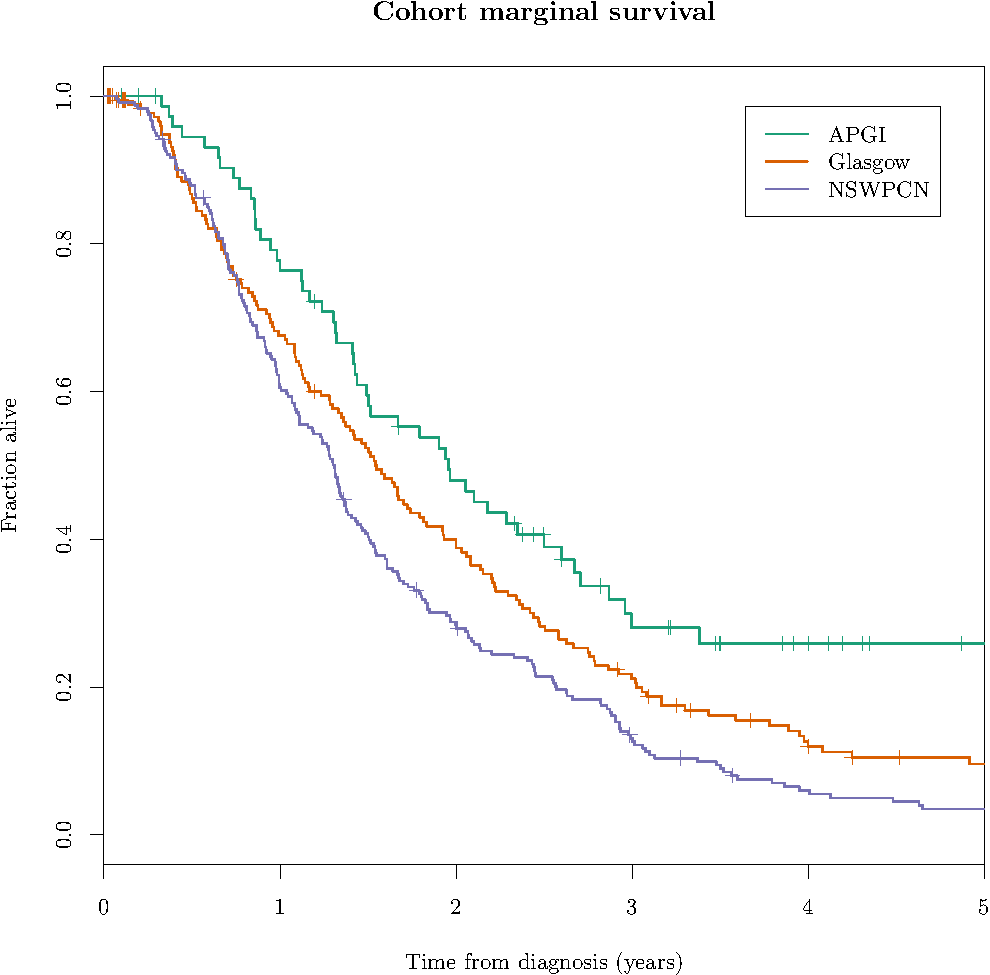
\includegraphics[width=.7\textwidth]{analysis/nomogram/figure/07-cohort-surv-comparison-1}
\caption[Cohort marginal survival estimates]{Kaplan-Meier marginal survival estimates for the cohorts used in this chapter.  Censoring times are indicated by $+$ symbols.}
\label{fig:nomo-cohort-km}
\end{figure}

\subsection{Prognostic model building and selection}
Candidate prognostic models were constructed on the \gls{NSWPCN} training data by iterative model fitting, evaluation, and refinement.  To guard against overfitting caused by this iterative process, the \gls{NSWPCN} cohort was randomly split once, into model building and testing sets.  All model fitting and refinement described below was performed on the 200-patient model building set, to yield three final candidate prognostic predictors.  The performance of each of these three predictors was then assessed on the 49-patient model test set, and the most parsimonious high-performing model was chosen as the \gls{PCOP} prognostic predictor, for subsequent external validation.

\paragraph{Cohort shift}
The \gls{NSWPCN} training cohort was collected over a long period, with patient diagnosis dates spanning the thirteen years from 1994 to 2006.  Over such an extended interval, subtle changes in cohort composition or therapy may cause a shift in cohort characteristics, and reduce the prognostic performance of a model that was built on the historical data, when it is applied to contemporary cases.  Cohort shift was investigated by examining the association between date of diagnosis, and all prognostic and outcome variables: in the absence of shift, no variables would be expected to change significantly over time.  Date of diagnosis was not significantly associated with any other variable, or outcome (distance correlation~\cite{Szekely2013} and \gls{CPH} regression, 7 tests, lowest $P = 0.35$); there was therefore no indication of cohort shift in the \gls{NSWPCN} training data.

\paragraph{Model functional form and expanded terms}
The \gls{CPH} framework was used to assess functional form for the two continuous covariates: age at diagnosis, and maximum pathological axis size.  \Gls{LOESS} smooths of martingale residuals~\cite{Therneau1990} indicated a largely linear relationship for age at diagnosis (\fref{fig:nomo-funcform-age}), and a knee-shaped form for size (\fref{fig:nomo-funcform-size}), with the knee at approximately $0$ in median-centered units.  In subsequent fits this potential nonlinear size effect was modelled by adding a $\mathrm{size}_+$ ramp term.  The original set of five linear prognostic terms, plus the additional nonlinear size term, was denoted the expanded term set.

\begin{figure}[!htbp]
\centering
  \subbottom[Patient age (centered)]{
    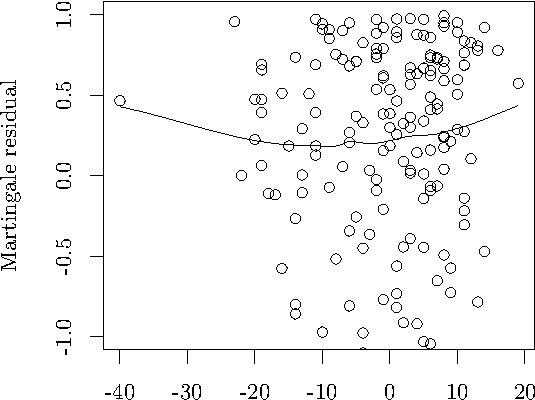
\includegraphics[width=.45\linewidth]{analysis/nomogram/figure/05-eda-func-form-age-2}
    \label{fig:nomo-funcform-age}}
  \subbottom[Tumour size (centered)]{
    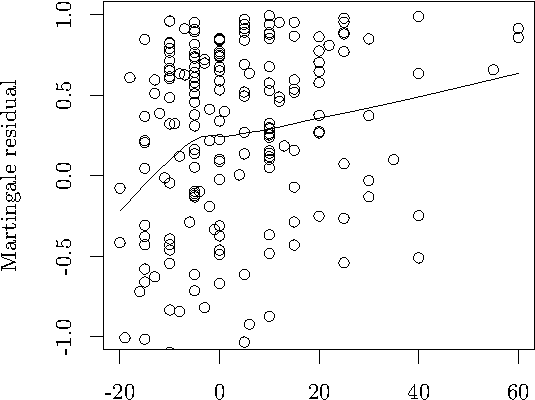
\includegraphics[width=.45\textwidth]{analysis/nomogram/figure/05-eda-func-form-size-2}
    \label{fig:nomo-funcform-size}}
\caption[Prognostic predictor functional forms]{\gls{NSWPCN} prognostic predictor functional forms. Smoothed Cox model martingale residual plots indicate hazard relationships that are approximately linear for centered age (panel a), and piecewise linear for centered tumour size (panel b).  For clarity, plots have been restricted to the residual range $[-1,1]$.}
\label{fig:nomo-funcform}
\end{figure}

\paragraph{Proportional hazards assumption}
A Grambsch-Therneau test~\cite{Grambsch1994} on the \gls{CPH} model fit using all expanded terms indicated that patient sex violated the \glspl{PH} assumption ($P = 0.0104$, \fref{fig:nomo-ph-plot-sex}) -- in other words, the two sexes had significantly different baseline hazard shapes.  To account for this effect, all subsequent models were stratified by patient sex, so that the survival of male and female patients was modelled by two different baseline hazard functions.  A Grambsch-Thernau test on the stratified model indicated no further significant violations of the \gls{PH} assumption (global $P = 0.4194$).

\begin{figure}[!htbp]
\centering
  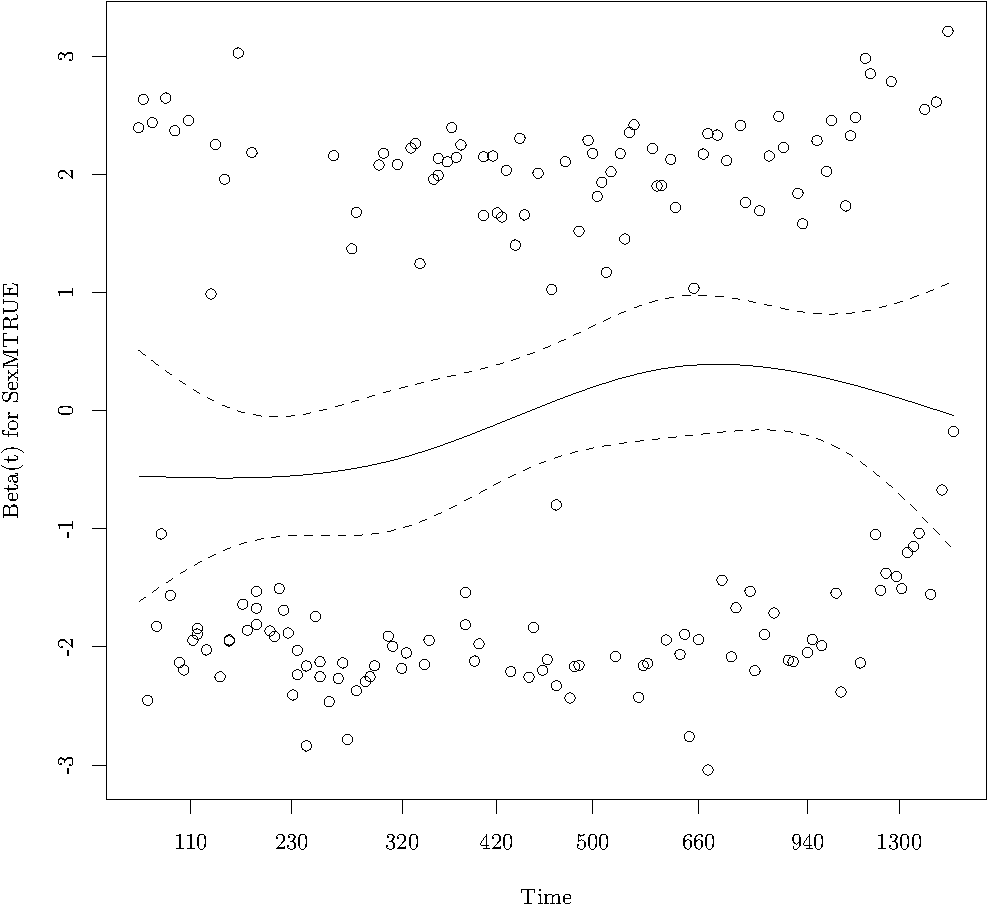
\includegraphics[width=.7\linewidth]{analysis/nomogram/figure/05-eda-ph-check-full-1}
  \caption[Baseline hazard forms differ between patient sexes]{NSWPCN baseline hazard differs between patient sexes.  A natural spline smooth of scaled Schoenfeld residuals for patient sex has a slope obviously differing from zero, suggesting that the baseline hazard forms differ between the two sexes, and that the combined data violates the \acrshort{PH} assumption of Cox regression.  Individual residuals are displayed as points, the natural spline smooth ($\mathrm{df}=4$) as a solid line, and approximate $\pm 1\ \mathrm{SE}$ bounds as dashed lines.}
\label{fig:nomo-ph-plot-sex}
\end{figure}

\paragraph{Outlier removal}
Strongly influential or outlying samples from the full marginal Cox fit were removed from the \gls{NSWPCN} building set.  I considered this unusual measure to be necessary given known and unresolvable quality issues in the \gls{NSWPCN} cohort data.  For all subsequent work, patients with full marginal Cox model absolute deviance residuals exceeding 2.5, or any absolute DFBETAS score exceeding 0.3, were excluded from the original building set.  This filter removed seven patients, reducing the size of the model building set to 193 patients.	

\paragraph{Variable selection}
Stepwise variable elimination was used to select an \gls{AIC}-optimal model starting from the full marginal \gls{CPH} model, containing all expanded terms and a sex stratum.  The identified optimal \gls{CPH} model used four variables: tumour location (head vs body), tumour size (linear term only), S100A2 status, and S100A4 status, in addition to the sex stratum.  The \gls{AIC}-selected set of four prognostic terms, and a patient sex stratum, was denoted the reduced term set.

\paragraph{Model CP1}
A final prognostic \acrshort{CPH} regression model was fit to the outlier-removed \gls{NSWPCN} model building data using only the reduced term set; this model was termed CP1.  CP1 did not violate the \gls{PH} assumption by the Grambsch-Therneau test (global $P = 0.794$).  Predictions from model CP1 were broadly concordant with stratified \gls{KM} estimates across all covariate subgroups, indicating no serious lack of fit of the model (\fref{fig:nomo-cp1-gg1-fitplot}).

\paragraph{Model GG1}
Semiparametric Cox \gls{PH} models such as CP1 provide a convenient framework for covariate testing and model diagnostics, but their unspecified baseline hazard term significantly complicates their use as prognostic predictors: patients are naturally only scored for relative hazard, and estimates of survival probabilities are unavailable.  Although it is possible to approximate the baseline hazard in the Cox model, a more natural alternative is to use fully parametric models, in which the baseline hazard distribution is explicity specified.  The advantages of parametric models in terms of robustness and interpretability are offset by their more stringent assumptions: if the chosen baseline distribution is unsuited to the particular data to be fit, predictions from parametric models can be very poor.  Given the potential benefits of parametric models for survival prediction, a parametric alternative to model CP1 was developed, and its fit assessed.  This parametric model was termed GG1.

Model GG1, employing a \gls{GG} survival distribution~\cite{Cox2007}, was fit to the outlier-removed \gls{NSWPCN} model building data by maximum likelihood.  Guided by the model functional form and baseline hazard stratification indicated by the Cox model diagnostics, the \gls{GG} distribution location parameter $\beta$ was made linearly dependent on all terms in the reduced set, but the shape parameters $\sigma$ and $\lambda$ were modelled as dependent on patient sex only.  Graphical comparisons between GG1 predictions and \gls{KM} estimates of survival indicated that GG1 predicted outcome to within error across major patient subgroups (\fref{fig:nomo-cp1-gg1-fitplot}).

\begin{figure}[!htbp]
\centering
  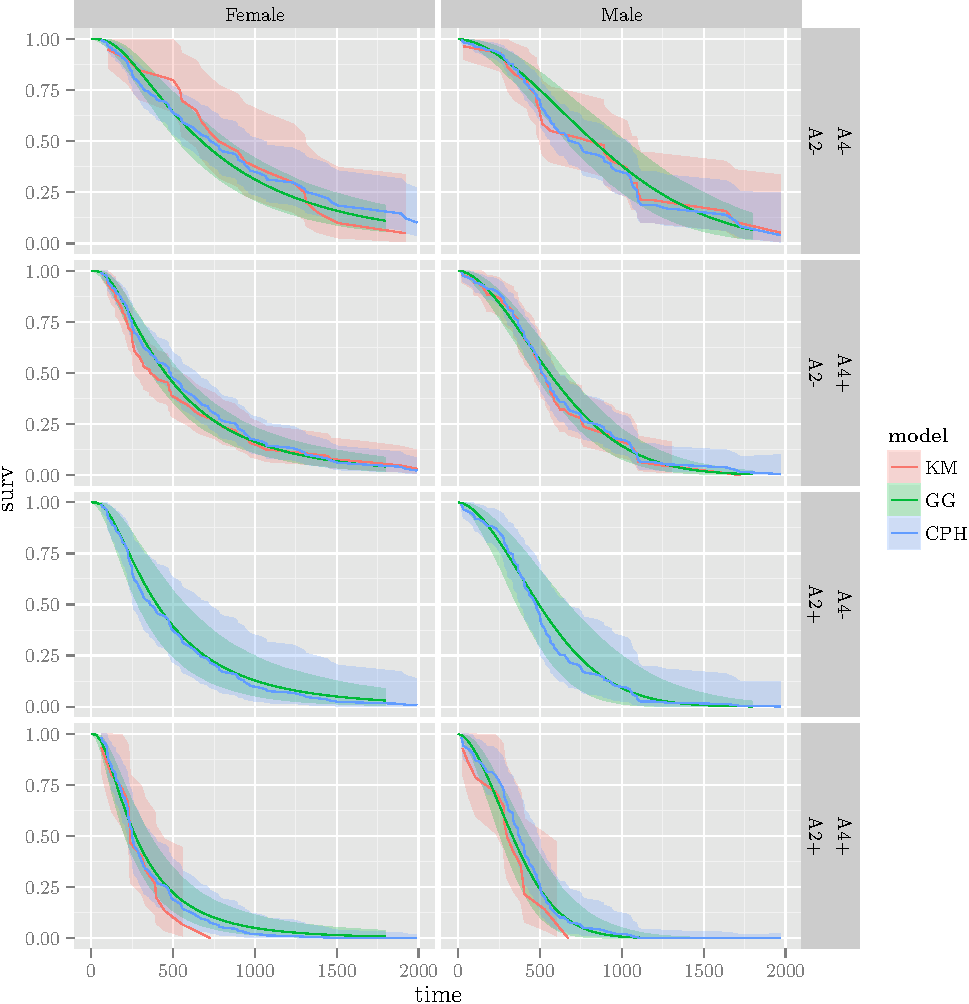
\includegraphics[width=.85\linewidth]{analysis/nomogram/figure/05-final-fit-assessment-2}
  \caption[Model survival predictions agree with stratified \texorpdfstring{\acrshort{KM}}{KM} estimates]{Model survival predictions agree with stratified \gls{KM} estimates.  \gls{KM} estimates of survival probability for each combination of patient sex and biomarker status are shown as solid red lines, with 95\% confidence intervals indicated by red ribbons.  Estimates of survival probability generated by models CP1 (blue), GG1 (green), and RSF (purple), broadly followed the form of the \gls{KM} estimator, and lay within its bounds at all times, although all models consistently overestimated survival of the double positive subgroup.  Both model fitting and prediction used the \gls{NSWPCN} model building set, and so these plots illustrate model goodness-of-fit, but cannot indicate possible overfitting.  \gls{KM} traces for the S100A2 positive, S100A4 negative group were omitted, as there were insufficient patients in this group for reliable \gls{KM} estimates to be available.  For all plots, tumour location, and size, were set to cohort median values.}
\label{fig:nomo-cp1-gg1-fitplot}
\end{figure}

\paragraph{Model RSF}
Regression models like CP1 and GG1 are familiar and readily interpretable, but are heavily dependent on the analyst identifying appropriate variables and functional forms.  Ensemble tree models such as random forests~\cite{Breiman2001} naturally and automatically model nonlinearity and arbitrary level interactions, and are tolerant of large numbers of irrelevant or collinear variables, albeit at the cost of very poor interpretability, and large data and computational requirements.  Random forests have been adapted to model censored data~\cite{Ishwaran2008}, and can provide an alternative prognostic predictor that is distinct in behaviour from CP1 and GG1, and may be able to exploit data structure not leveraged by these more classical models.

To investigate whether tree ensemble models could provide improved performance over classical approaches, a random survival forest model, termed RSF, was fit to the outlier-removed \gls{NSWPCN} model building data.  In contrast to CP1 and GG1, which used the reduced set of terms as covariates, RSF was supplied all preoperatively-assessable variables as candidate predictors.

\paragraph{Model selection}
Predictive performance of the three prognostic models (CP1, GG1, and RSF) was compared on the holdout \gls{NSWPCN} model test set, to select a single high-performing parsimonious model for external validation.  Model discriminatory ability was assessed over time using the \gls{AUC} of the incident/dynamic \gls{TDROC}~\cite{Heagerty2005}, and overall prognostic accuracy (combining both discrimination and calibration) over time by the Brier score~\cite{Graf1999}.  The integrated Brier score~\cite{Graf1999} was also used to provide an aggregate measure of overall model accuracy.  Performance in the interval from seven to 34 months post-diagnosis was of particular interest, as the majority of patients in the \gls{NSWPCN} training set died during this period (\fref{fig:nomo-cohort-km}).

All models had statistically indistinguishable discriminatory power over the $7-34$ month period, as assessed by pointwise $95\%$ BCa confidence intervals~\cite{Efron1987} of the \gls{TDROC} \gls{AUC} (\fref{fig:nomo-tdauc-paths}).  There was also no significant difference between candidate models in Brier score, integrated over $7-34$ months, although all models performed significantly better than a marginal Kaplan-Meier prognostic, KM0 (\tref{tab:nomo-ibs-boot}).  Despite these non-significant differences, models GG1 and CP1 had consistently superior Brier score to RSF over the period of interest (\fref{fig:nomo-brier-paths}).  As there was no significant difference in performance between the prognostic models, the simplest model, GG1, was selected to form the \gls{PCOP}.

\begin{table}
\centering
\caption[Prognostic model \texorpdfstring{\acrshort{IBS}}{IBS} comparison]{Competing models do not have significantly different \gls{IBS} performance.  The \gls{IBS} is a combined measure of model predictive ability over a follow-up time interval, which captures both discrimination and calibration; lower numbers are better.  Differences in the $7-34$ month \gls{IBS} of competing models were calculated for each of 1,000 bootstrap samples of the \gls{NSWPCN} holdout test set, and $95\%$ BCa confidence intervals~\cite{Efron1987} calculated.  All candidate prognostic models had significantly better \gls{IBS} than the marginal KM0 model, but there was significant no difference between candidate models.  The $7-34$ month region in which most patients die is indicated by vertical black lines.}
\label{tab:nomo-ibs-boot}
\begin{tabular}{lrrr}
\toprule
                             & \multicolumn{2}{c}{Bootstrap}   \\ \cmidrule(r){2-3}
Comparison                   & Mean          & $95\%$ CI       \\ \midrule
$\mathrm{KM0} - \mathrm{GG1}$    & $21.1$        & $[2.5, 39.8]$   \\
$\mathrm{KM0} - \mathrm{CPH}$    & $20.2$        & $[4.5, 38.9]$   \\
$\mathrm{KM0} - \mathrm{RSF}$    & $14.5$        & $[5.7, 24.6]$   \\
$\mathrm{RSF} - \mathrm{GG1}$    &  $6.6$        & $[-5.6, 17.7]$  \\
$\mathrm{RSF} - \mathrm{CPH}$    &  $5.7$        & $[-2.9, 15.9]$  \\ 
$\mathrm{CPH} - \mathrm{GG1}$    &  $0.9$        & $[-4.1, 4.3]$   \\ \bottomrule
\end{tabular}
\end{table}

\paragraph{Final \texorpdfstring{\acrshort{PCOP}}{PCOP} fit}
A final fit of GG1 to the full \gls{NSWPCN} training data (both model building and validation patients) was made, and is summarised in \tref{tab:nomo-final-fit}.  This fit defined the \gls{PCOP}, which predicts post-resection outcome using a generalized gamma model~\cite{Cox2007}, as
\begin{align*}
T \sim GG(\beta   = &\ 6.7446 + 0.3732[\mathrm{Sex = Male}] - 0.2150[\mathrm{Location = Body}] \\
                    &\ -0.0887\;\mathrm{Size} - 0.3729[\mathrm{S100A2 = Positive}] \\
                    &\ -0.3843[\mathrm{S100A4 = Positive}], \\ 
          \sigma  = &\ 0.7503 - 0.2452[\mathrm{Sex = Male}],\\
          \lambda = &\ 0.0288 - 0.7630[\mathrm{Sex = Male}])
\end{align*}
where $T$ is an individual's failure time, $GG$ is the generalized gamma distribution, $\mathrm{Size}$ is in centimetres, and $[\;]$ is the Iverson bracket.

\begin{figure}[!htbp]
\centering
  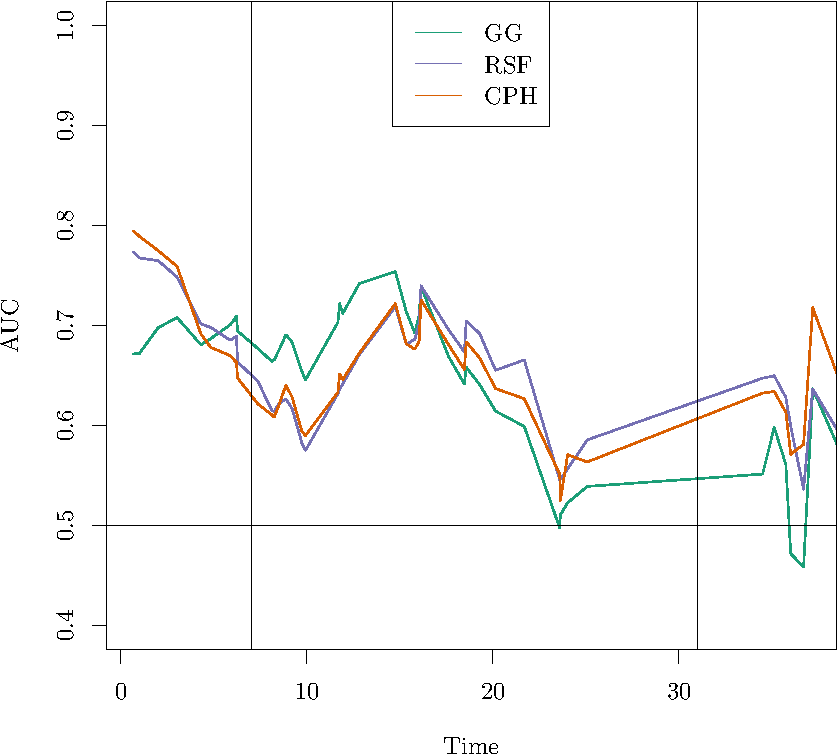
\includegraphics[width=.7\linewidth]{analysis/nomogram/figure/05-model-selection-roc-id-1}
  \caption[Time-dependent \texorpdfstring{\acrshort{AUC}}{AUC} paths for candidate models on holdout data]{Incident / dynamic \gls{TDROC} \gls{AUC} paths for candidate models on the holdout \gls{NSWPCN} model test set.  Slight differences in performance were evident, with model GG1 providing superior discrimination up to approximately 15 months post-diagnosis, but models RSF and CP1 performing better from approximately 20 months post-diagnosis.  These differences were not significant, as assessed by pointwise $95\%$ bootstrap confidence intervals (confidence bands not shown).  The $7-34$ month interval in which most patients died is indicated by dashed vertical lines.}
\label{fig:nomo-tdauc-paths}
\end{figure}

\begin{figure}[!htbp]
\centering
  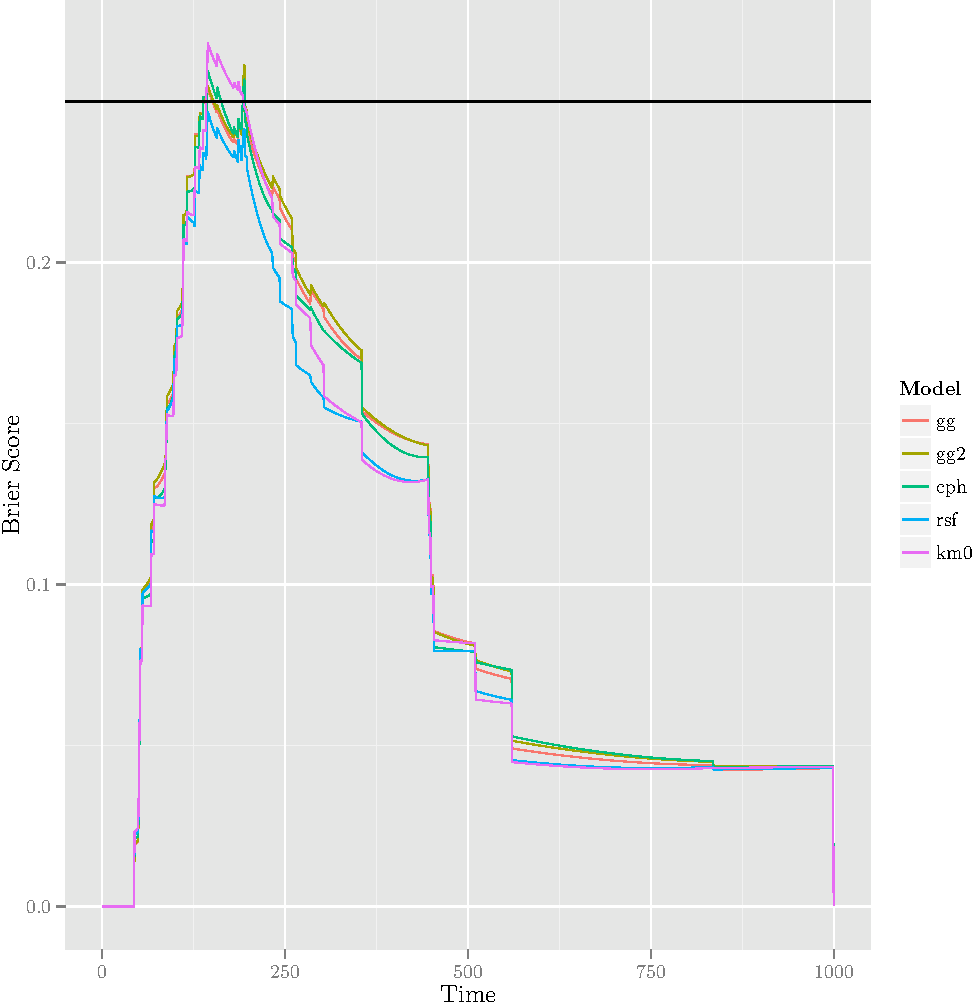
\includegraphics[width=.7\linewidth]{analysis/nomogram/figure/05-model-selection-bs-paths-1}
  \caption[Brier score paths for candidate models on holdout data]{Brier score paths for candidate models on the holdout \gls{NSWPCN} model test set.  All models outperformed the no-information KM0 trace from approximately four months to 21 months post-diagnosis, and no strong differences were apparent between candidate models.  The $7-34$ month interval in which the majority of patients died is indicated by dashed lines, and the theoretical worst-case Brier score by a horizontal line at $0.25$.}
\label{fig:nomo-brier-paths}
\end{figure}


\begin{table}
\centering
\caption[Final PCOP fit]{Coefficients of a final GG1 fit to the \gls{NSWPCN} training data, which defines the \gls{PCOP}.  Coefficient estimates are for a generalized gamma survival model~\cite{Cox2007}.}\label{tab:nomo-final-fit}
\begin{tabular}{llrr}
\toprule
Term                   &                & Estimate       & SE       \\ \midrule
$\beta$ \\
(Intercept)            &                &  $6.7446$      & $0.1489$ \\
Sex                    & = Male         &  $0.3732$      & $0.1508$ \\
Tumour location        & = Body         & $-0.2150$      & $0.1223$ \\
Size of longest axis   &  (cm)          & $-0.0887$      & $0.0302$ \\
S100A2                 & = Positive     & $-0.3729$      & $0.1235$ \\
S100A4                 & = Positive     & $-0.3843$      & $0.1045$ \\[10pt]
$\sigma$ \\
(Intercept)            &                &  $0.7503$      & $0.0493$ \\
Sex                    & = Male         & $-0.2452$      & $0.1066$ \\[10pt]
$\lambda$ \\
(Intercept)            &                &  $0.0288$      & $0.2719$ \\
Sex                    & = Male         &  $0.7630$      & $0.3533$ \\[5pt] \bottomrule
\end{tabular}
\end{table}


\subsection{External validation}
Discrimination, calibration, and overall fit of the \gls{PCOP} was tested on three independent validation cohorts, following published guidelines~\cite{Royston2013}.

\subsubsection{Overall assessment of \texorpdfstring{\acrshort{PCOP}}{PCOP} fit}
\paragraph{Distribution of the \texorpdfstring{\acrshort{PCOP}}{PCOP} \texorpdfstring{\acrshort{PI}}{PI}}
Approximate \glspl{PI} for the \gls{PCOP} showed broadly similar distributions across the training \gls{NSWPCN} cohort, and the three validation cohorts (\fref{fig:nomo-score-hists}).  Vertical lines denote the empirical 20th, 50th, and 80th percentiles, which were also used to define risk groups to visually evaluate \gls{PCOP} fit.

\begin{figure}[!htbp]
\centering
  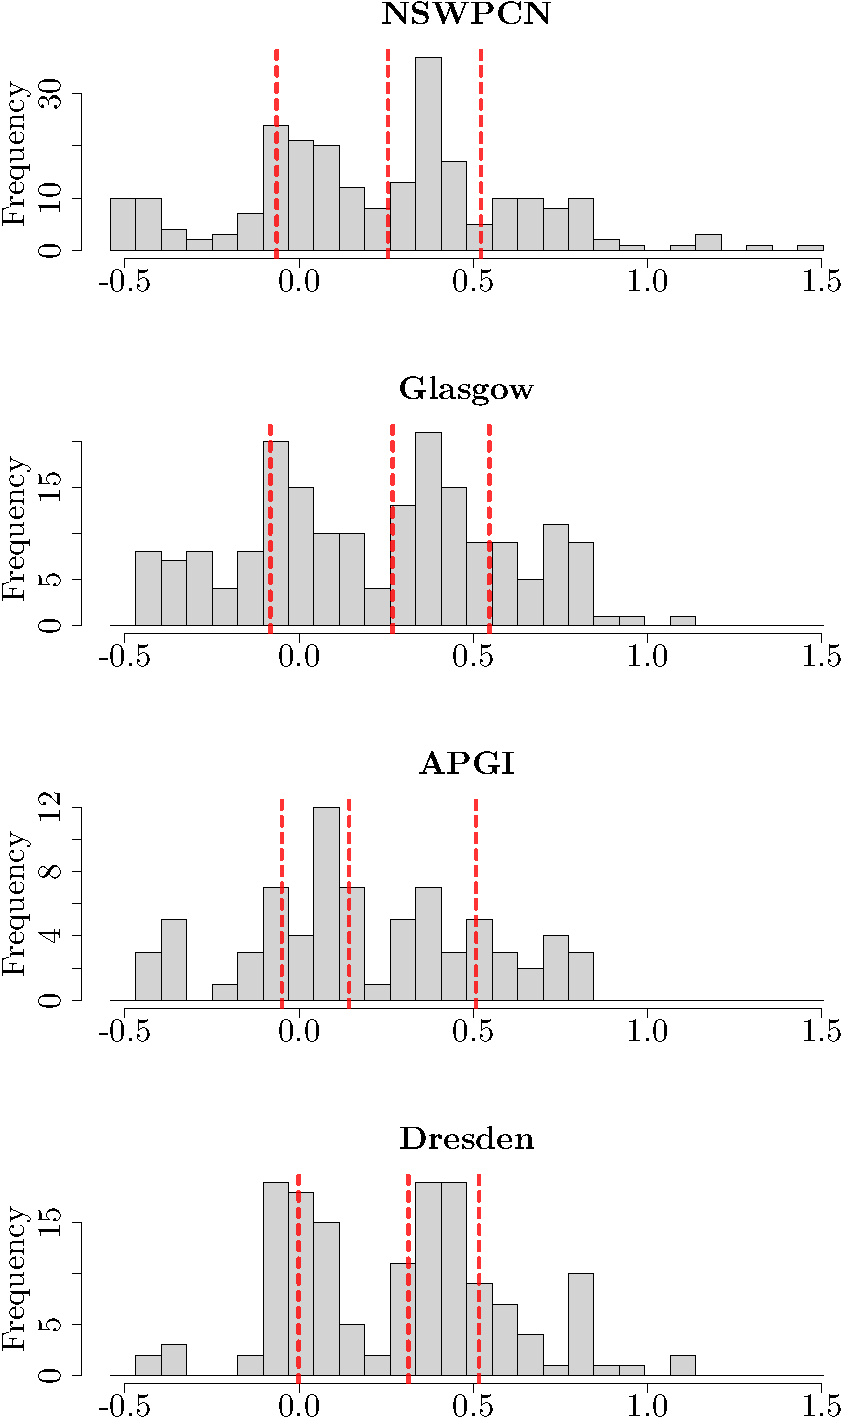
\includegraphics[width=.7\linewidth]{analysis/nomogram/figure/07-score-hists-1}
  \caption[\texorpdfstring{\acrshort{PCOP}}{PCOP} \texorpdfstring{\acrshort{PI}}{PI} distributions in training and validation cohorts]{Distributions of the \acrshort{PCOP} \acrshort{PI} in training and validation cohorts.  Score distributions were broadly similar in all cohorts, with an approximately bimodal form.  Empirical 20th, 50th, and 80th percentiles are indicated by red lines.}
\label{fig:nomo-score-hists}
\end{figure}

\paragraph{Visual assessment of \texorpdfstring{\acrshort{PCOP}}{PCOP} fit}
Patients within each cohort were divided into broad risk groups based on their \gls{PCOP} approximate \gls{PI}, and observed and predicted outcomes within each group were visually compared to evaluate model fit.  Three risk groups were defined: a high-risk group of patients with \gls{PI} less than the empirical cohort 20th percentile; a low-risk group with \gls{PI} greater than the 80th percentile; and an intermediate risk group with all remaining patients.  Overall model fit was good in the Glasgow validation cohort (\fref{fig:nomo-val-altman4-glasgow}), but poor in the \gls{APGI} and Dresden cohorts (\fref{fig:nomo-val-altman4-apgi}, \fref{fig:nomo-val-altman4-dresden}).  

\begin{figure}[!htbp]
\centering
  \subbottom[NSWPCN]{
    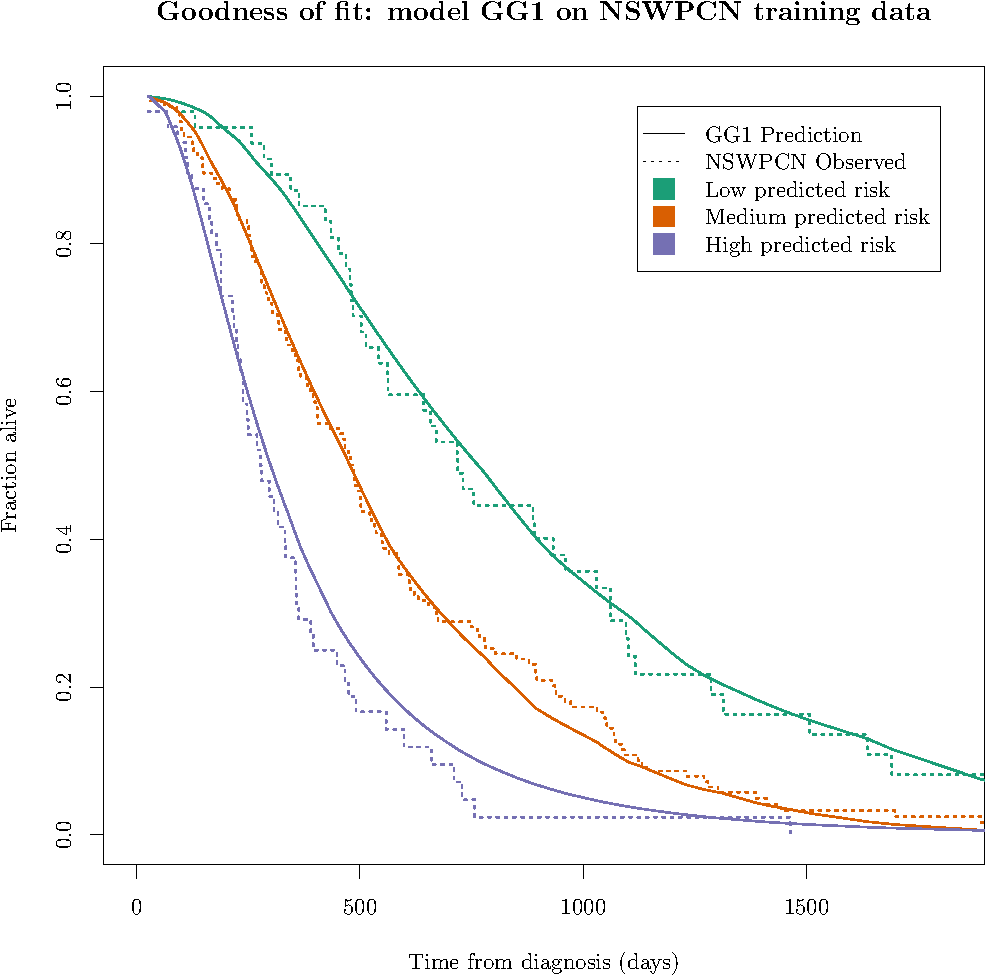
\includegraphics[width=.45\linewidth]{analysis/nomogram/figure/07-altman-4-nswpcn-1}
    \label{fig:nomo-val-altman4-nswpcn}}
  \subbottom[Glasgow]{
    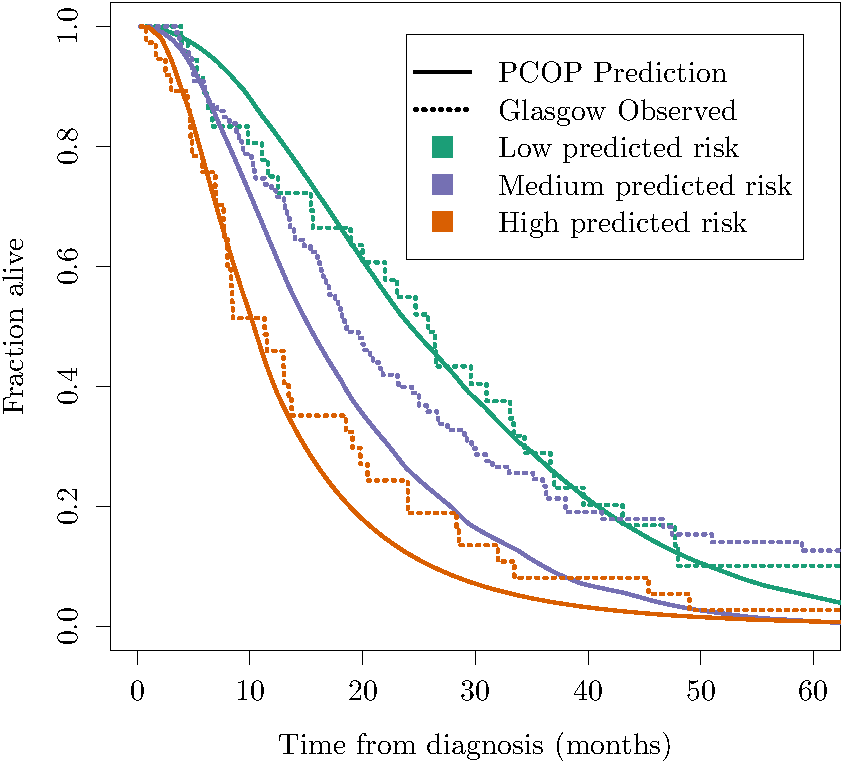
\includegraphics[width=.45\linewidth]{analysis/nomogram/figure/07-altman-4-glasgow-2}
    \label{fig:nomo-val-altman4-glasgow}}
  \subbottom[APGI]{
    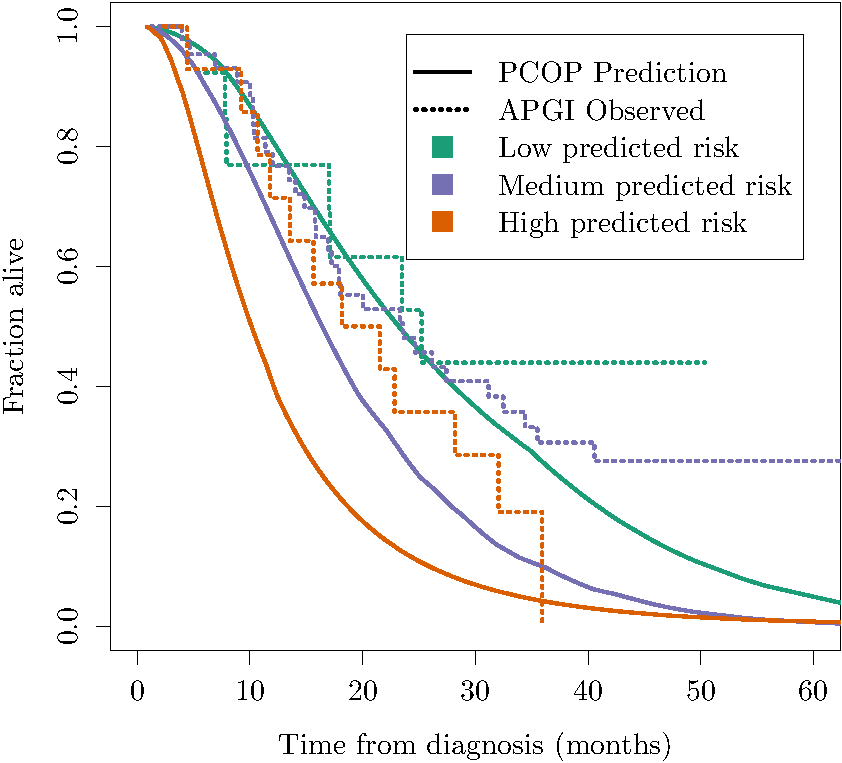
\includegraphics[width=.45\linewidth]{analysis/nomogram/figure/07-altman-4-apgi-2}
    \label{fig:nomo-val-altman4-apgi}}
  \subbottom[Dresden]{
    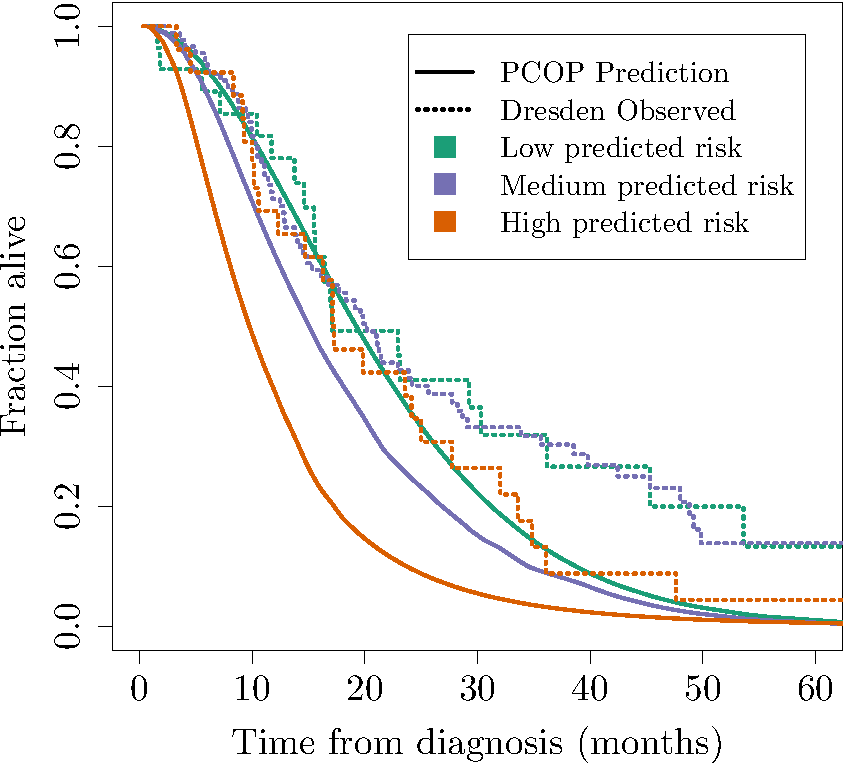
\includegraphics[width=.45\linewidth]{analysis/nomogram/figure/07-altman-4-dresden-2}
    \label{fig:nomo-val-altman4-dresden}}
\caption[Observed and predicted survival of patient risk groups]{Observed and \gls{PCOP} predicted survival of patient risk groups.  Within each cohort, patients were divided into three risk groups: high (red, \gls{PCOP} \gls{PI} $<$ 20th percentile), low (green, \gls{PI} $>$ 80th percentile), and medium (blue, all remaining patients).  For each group, a Kaplan-Meier estimate of empirical survival (dotted lines) was compared to the median of \gls{PCOP} predictions for patients in that group (solid lines).  Excellent fit is seen for the \gls{NSWPCN} training cohort, as expected.  Overall fit is poorer for the validation data, with acceptable fit for extreme risk groups in the Glasgow cohort, and generally poor fit in both the \gls{APGI} and Dresden cohorts.}
\label{fig:nomo-val-altman4}
\end{figure}

\paragraph{\texorpdfstring{\acrshort{PCOP}}{PCOP} Brier score}
The Brier score summarises overall model prediction error over time, without requiring patients to be divided into arbitrary risk groups based on approximate \gls{PI}.  To further investigate the poor fit observed in some cohorts, Brier score paths were calculated for the \gls{PCOP} in all three validation cohorts.  The performance of the \gls{MSKCC} nomogram, applied to preoperative variables, was also assessed at its three timepoints to provide a comparison between the \gls{PCOP} and an established prognostic tool.

\begin{figure}[!htbp]
\centering
  \subbottom[Glasgow]{
    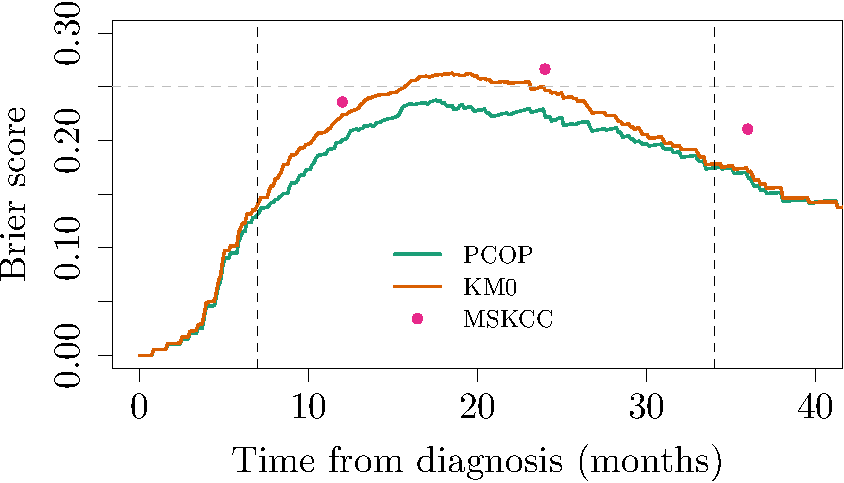
\includegraphics[width=.6\linewidth]{analysis/nomogram/figure/07-prob-bs-paths-plot-glasgow-1}
    \label{fig:nomo-val-brier-glasgow}}
  \subbottom[APGI]{
    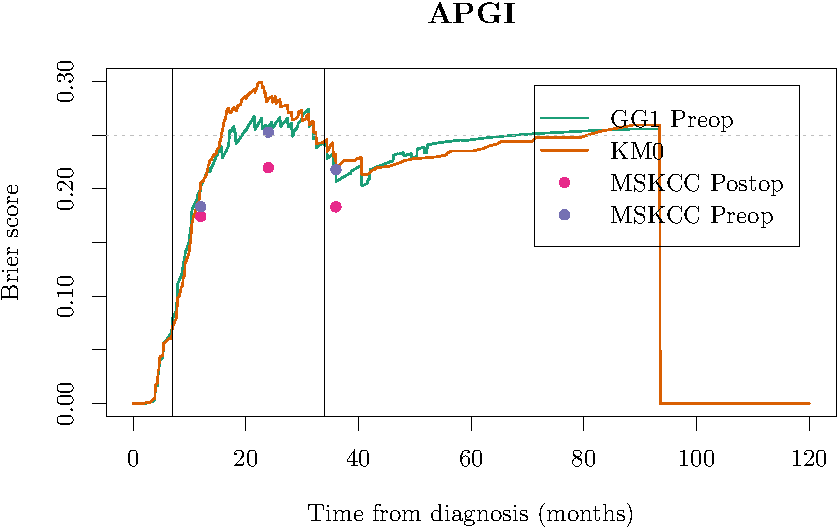
\includegraphics[width=.6\linewidth]{analysis/nomogram/figure/07-prob-bs-paths-plot-apgi-1}
    \label{fig:nomo-val-brier-apgi}}
  \subbottom[Dresden]{
    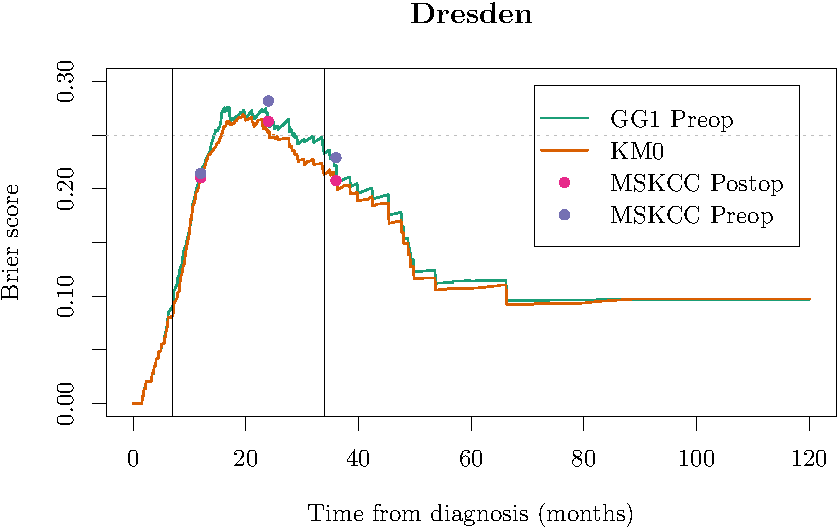
\includegraphics[width=.6\linewidth]{analysis/nomogram/figure/07-prob-bs-paths-plot-dresden-1}
    \label{fig:nomo-val-brier-dresden}}
\caption[Brier score paths for \texorpdfstring{\acrshort{PCOP}}{PCOP} on validation cohorts]{Brier score paths for \acrshort{PCOP} on validation cohorts.  The Brier score measures overall prognostic error, as a combination of calibration and discrimination; lower values are better, and the worst-case theoretical value is 0.25.  Brier score paths over time are shown for outcome predictions by \acrshort{PCOP} (green line), and the \acrshort{MSKCC} nomogram on preoperative data (pink dots).  Also shown is a marginal \acrshort{KM} prediction of outcome (orange), and the theoretical no-information Brier score limit (horizontal dotted line) -- outcome predictors must be substantially better than both of these to be usefully prognostic.  The $7-34$ month period in which most patients die is delimited by vertical lines.  \acrshort{PCOP} is substantially better than either the \acrshort{KM} or \acrshort{MSKCC} predictors in the Glasgow cohort, but all predictors are equally poor in the \acrshort{APGI} and Dresden cohorts.}
\label{fig:nomo-val-brier}
\end{figure}

In keeping with the general findings from visual assessment of risk groups, the \gls{PCOP} was more prognostic than null models in the Glasgow cohort, but not in the \gls{APGI} or Dresden cohorts, across all times post diagnosis (\fref{fig:nomo-val-brier}).  The significance of the difference between \gls{PCOP} and KM0 Brier score in the Glasgow cohort was assessed by bootstrapping, at 12, 24, and 36 months following diagnosis.  The \gls{PCOP} had a significantly better Brier score than KM0 at 24 months after diagnosis ($95\%$ BCa CI $[0.0024, 0.047]$, 500 rounds), but not 12 or 36 months.

The performance of the \gls{MSKCC} nomogram on preoperative data was poor: in all three cohorts, the performance of \gls{MSKCC} survival estimate was either not significantly different from, or was significantly worse than, that of the null KM0 model (\fref{fig:nomo-val-brier}).  The \gls{MSKCC} nomogram was designed exclusively for use with postoperative data, and it is reasonable to suppose that this is the reason for its poor performance on preoperative data.  However, when all postoperative data were supplied to the \gls{MSKCC} nomogram, its predictions also were not better than the null KM0 model in both the Glasgow and Dresden cohorts, suggesting either poor general discrimination or calibration of the \gls{MSKCC} nomogram in these data sets (data not shown).

\paragraph{Summary}
The \gls{PCOP} demonstrated acceptable overall fit in only one of the three validation cohorts tested.  Poor fit can be caused by both model miscalibration, and poor discrimination.  Miscalibration of a prognostic model, while not ideal, does not preclude its clinical use~\cite{Steyerberg2010}: if discrimination remains good, the model can still be used to place patients into risk groups, which inform decision making.  On the other hand, if a model shows very poor discrimination, it is generally meaningless.  The clinical utility of the \gls{PCOP} was evaluated by formally testing its discrimination, separately from calibration, in the validation cohorts.

\subsubsection{Discrimination}
Discrimination of the \gls{PCOP} on external cohorts was assessed by Harrell's $c$-index~\cite{Harrell1982}, calibration slope tests, and the incident / dynamic \gls{TDROC}~\cite{Heagerty2005}.

\paragraph{\texorpdfstring{$c$}{c}-index}
Harrell's $c$-index is defined as the proportion of patients for which the \gls{PI} and outcome are concordant: in other words, the empirical probability that, for a randomly chosen pair of patients in a cohort, the one with the higher \gls{PI} will die sooner.  As such, the $c$-index is an overall measure of the ability of a given \gls{PI} to discriminate between patients with different outcome.  Values of the $c$-index for the \gls{PCOP} and preoperative \gls{MSKCC} \glspl{PI} were calculated in each validation cohort, and are summarised in table \tref{tab:nomo-val-hcis}.  In the Glasgow cohort, the \gls{PCOP} was $c$-index was significantly better than that of a marginal predictor (Penciana test~\cite{Penciana2004} $P = 6.67 \times 10^{-6}$), and was also significantly better than the \gls{MSKCC} preoperative nomogram $c$ ($P = 0.041$).  In the remaining two cohorts, both the \gls{PCOP}, and the \gls{MSKCC} preoperative nomogram, showed very poor overall discrimination.

\begin{table}[!htbp]
\centering
\caption[Harrell \texorpdfstring{$c$}{c}-indices for \texorpdfstring{\acrshort{PCOP}}{PCOP} in validation data]{Harrell's $c$-indices for \gls{PCOP} and preoperative \gls{MSKCC} \glspl{PI} in validation cohorts.  Values of Harrell's $c$, and associated P-values testing whether $c$ is significantly different from the no-information value of 0.5 ($P_{0.5$}), are given for both the \gls{PCOP}, and the \gls{MSKCC} nomogram applied to preoperative data.  Both \glspl{PI} are significantly prognostic in the Glasgow cohort, and only weakly so, if at all, in the \gls{APGI} and Dresden cohorts.}\label{tab:nomo-val-hcis}
\begin{tabular}{@{}lllll@{}}
\toprule
          & \multicolumn{2}{c}{PCOP}           & \multicolumn{2}{c}{MSKCC}            \\ 
\cmidrule(r){2-3} \cmidrule(r){4-5}
Cohort    & $c$     & $P_{0.5}$                & $c$        & $P_{0.5}$               \\ \midrule
Glasgow   & 0.609   & $6.67 \times 10^{-6}$    & 0.585      & $6.96 \times 10^{-4}$   \\
APGI      & 0.580   & $0.045$                  & 0.476      & $0.55$                  \\
Dresden   & 0.546   & $0.124$                  & 0.518      & $0.50$                  \\ \bottomrule
\end{tabular}
\end{table}

\paragraph{Tests of `calibration slope'}
A common approach to test a prognostic model's fit and discrimination on test data is to verify that a \gls{PI} derived from the model is significantly prognostic when it is used as the sole predictor in a Cox model, and that the \gls{PI} coefficient is not significantly different from unity.  This validation method was applied to both the \gls{PCOP} and preoperative \gls{MSKCC} prognostics, on the three validation data sets.  The \gls{PCOP} passed this validation test in both the Glasgow and \gls{APGI}, but not the Dresden, cohorts, and the preoperative \gls{MSKCC} did not validate in any cohort (\tref{tab:nomo-val-slope}).  Despite its validating in two cohorts, the fitted \gls{PCOP} \gls{PI} coefficient was consistently less than one, suggesting that overfitting occurred during construction of the \gls{PCOP}~\cite{Royston2013}.

\begin{table}[!htbp]
\centering
\caption[Tests of \texorpdfstring{\acrshort{PCOP}}{PCOP} calibration slope]{Calibration slope tests of the \gls{PCOP} and \gls{MSKCC} \gls{PI}.  Coefficients ($\beta$) of Cox model fits using either the \gls{PCOP} or preoperative \gls{MSKCC} \gls{PI} as sole predictor are given, along with P-values testing whether the coefficients are significantly different from both zero ($P_0$), and one ($P_1$).  A \gls{PI} that passes the test will have results consistent with $\beta = 1$.  The \gls{PCOP} satisfies this requirement for the Glasgow and \gls{NSWPCN} cohorts, but not the Dresden cohort.  The \gls{MSKCC} nomogram, when applied to preoperative data, fails in all three cohorts.  Despite the successful validation of the \gls{PCOP} in two cohorts, its regression coefficients are consistently smaller than 1, suggesting that the \gls{PCOP} model was overfit during training.}\label{tab:nomo-val-slope}
\begin{tabular}{@{}llllll@{}}
\toprule
          & \multicolumn{3}{c}{PCOP}     & \multicolumn{2}{c}{MSKCC}  \\ \cmidrule(r){2-4} \cmidrule(r){5-6}
Cohort    & $\beta$  & $P_0$   & $P_1$   & $\beta$    & $P_0$         \\ \midrule
Glasgow   & 0.805    & 0.001   & 0.41    & 0.012      & 0.284         \\
APGI      & 0.894    & 0.036   & 0.80    & 0.003      & 0.634         \\
Dresden   & 0.527    & 0.093   & 0.13    & 0.003      & 0.502         \\ \bottomrule
\end{tabular}
\end{table}

\paragraph{Incident / dynamic \texorpdfstring{\acrshort{TDROC}}{TD-ROC}}
Both the $c$-index and calibration slope tests provide single measures of model discrimination, averaged across all observed times.  However, a prognostic model's discrimination is not generally constant, but changes over time, and it is possible that a model with poor average performance could have good discrimination at specific follow-up times.  To address this, plots of \gls{TDROC} \glspl{AUC} were used to assess the \gls{PCOP}'s discriminative ability at a range of times after diagnosis.

In both the Glasgow and \gls{APGI} cohorts, the \gls{PCOP} displayed consistently better discrimination than a null model, and the \gls{MSKCC} nomogram on preoperative data, for a range of times after diagnosis (\fref{fig:nomo-val-tdroc}).  This result was not repeated in the Dresden cohort, for which both the \gls{PCOP} and the \gls{MSKCC} nomogram displayed discrimination that was barely better than baseline.

\begin{figure}[!htbp]
\centering
  \subbottom[Glasgow]{
    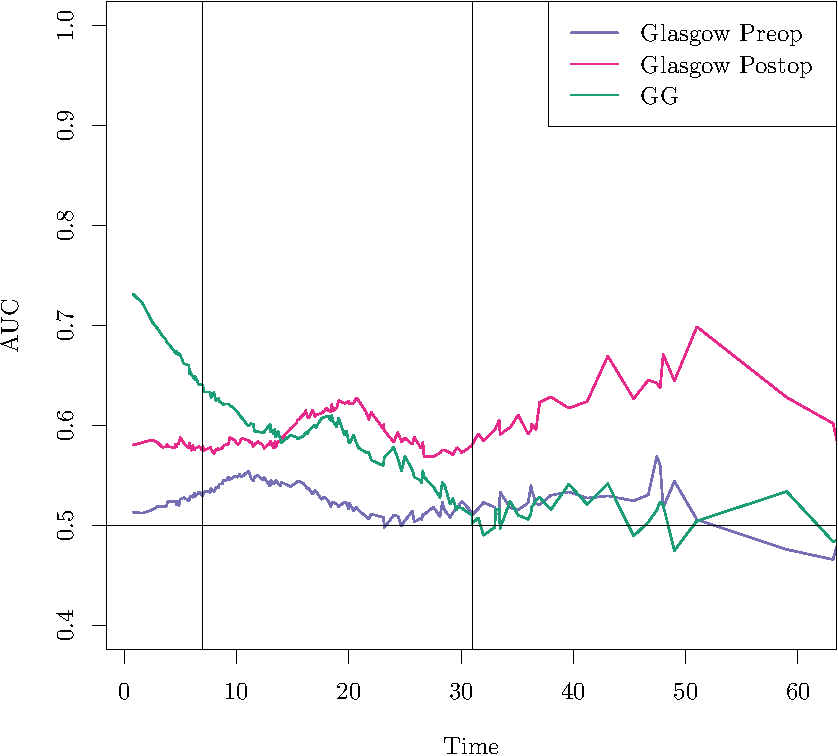
\includegraphics[width=.6\linewidth]{analysis/nomogram/figure/07-risksetROC-plot-glasgow-1}
    \label{fig:nomo-val-tdroc-glasgow}}
  \subbottom[APGI]{
    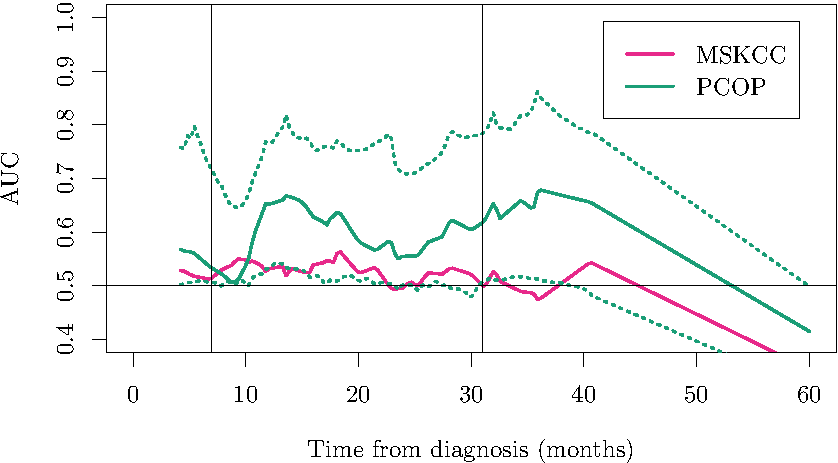
\includegraphics[width=.6\linewidth]{analysis/nomogram/figure/07-risksetROC-plot-apgi-1}
    \label{fig:nomo-val-tdroc-apgi}}
  \subbottom[Dresden]{
    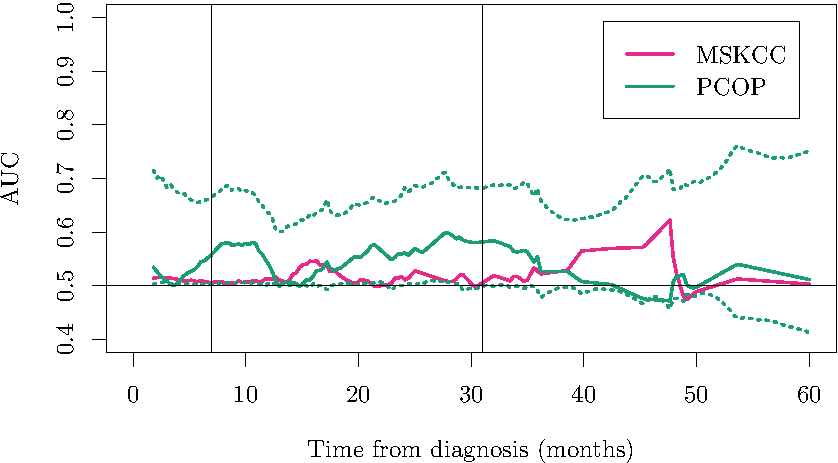
\includegraphics[width=.6\linewidth]{analysis/nomogram/figure/07-risksetROC-plot-dresden-1}
    \label{fig:nomo-val-tdroc-dresden}}
\caption[\texorpdfstring{\acrshort{TDROC}}{TD-ROC} \texorpdfstring{\acrshort{AUC}}{AUC} paths for \texorpdfstring{\acrshort{PCOP}}{PCOP} in validation data]{\gls{TDROC} \gls{AUC} over time in validation cohorts.  Bootstrap summaries of the \gls{AUC} are shown for \glspl{PI} from the \gls{PCOP} (mean: green solid lines; BCa $95\%$ confidence intervals: green dotted lines), and the \gls{MSKCC} nomogram on preoperative data (mean: red lines).  The \gls{PCOP} displays consistently superior discrimination to the no-information level (horizontal line at $0.5$) in the Glasgow and \gls{APGI} cohorts, but performs much more poorly in the Dresden cohort.  The \gls{MSKCC} nomogram \gls{PI} performs poorly in all cohorts.  Vertical dashed lines indicate the $7-34$ month region in which most patients die.}
\label{fig:nomo-val-tdroc}
\end{figure}

\subsubsection{Validation summary}
A range of complementary validation approaches were applied to test the performance of the \gls{PCOP} in external validation cohorts.  In terms of overall fit, the \gls{PCOP} was superior to null models in the Glasgow cohort, but not in the \gls{APGI} or Dresden cohorts.  Specific tests of discrimination were used to check if the poor overall fit was due to poor model discrimination, and indicated that the \gls{PCOP} discriminated between good- and poor-prognosis patients well in the Glasgow and \gls{APGI} cohorts, but poorly in the Dresden cohort.  The preoperative \gls{MSKCC} nomogram was a poor prognostic in all data sets.

\subsection{PCOP web application}
A serious barrier to the use of complex prognostic tools such as the \gls{PCOP} is the difficulty in their calculation.  To address this, a simple web application was created to encapsulate the \gls{PCOP}, and allow its easy evaluation from any web browser.  The \gls{PCOP} web application interface is illustrated in \fref{fig:nomo-web-example}.  In response to user input of basic clinical parameters, the web interface dynamically recalculates survival estimates, and returns them in graph and table form.  Up to two survival curves may be shown simultaneously, to allow the easy comparison of cases.  The demonstration \gls{PCOP} web application resides on the \gls{AWS} framework, and so is straightforward to deploy both publicly, and privately, as required.

A demonstration instance of the \gls{PCOP} web application is available at \url{http://www.pancpredict.net:3277/}.\mpfatal{Update the web app with the final PCOP}

\begin{figure}[!htbp]
\centering
  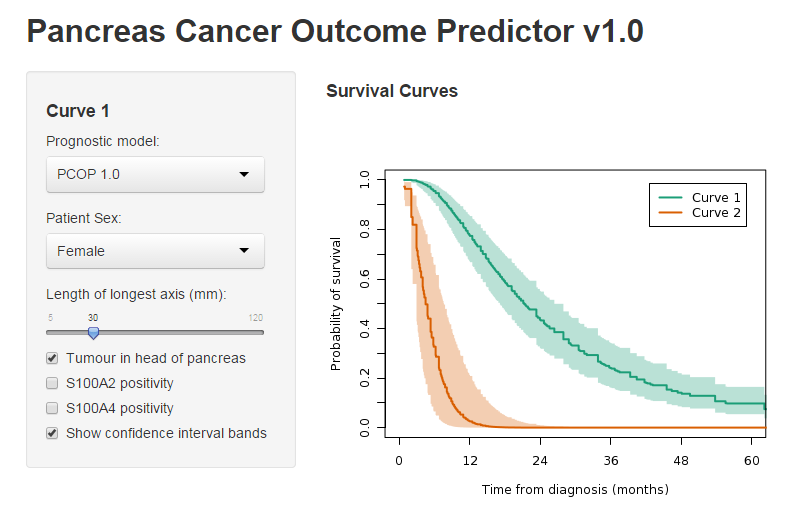
\includegraphics[width=1\linewidth]{analysis/nomogram/webapp/PCOP.png}
\caption[Example screenshot of the \texorpdfstring{\acrshort{PCOP}}{PCOP} web application]{Example screenshot of the \gls{PCOP} web application.  The user enters clinical data for up to two cases, and the system dynamically calculates and displays predicted survival curves, optionally with confidence bands.}
\label{fig:nomo-web-example}
\end{figure}

\section{Discussion}
Is it possible to create a clinically useful preoperative prognostic tool for pancreas cancer?  This chapter's work aimed to address part of that question, by developing and validating the \gls{PCOP}, a prognostic for resected pancreas cancer that uses postoperative measurements as surrogates for preoperative ones.  The \gls{PCOP} validated in one external cohort, but not two others, and the question remains as to whether it, or a true preoperative prognostic based upon it, would ultimately have any clinical utility.  Cohort differences and likely confounding were the ultimate cause of the poor validation performance of the \gls{PCOP}, with the substantial differences between cohorts severely limiting the generalizability of \emph{any} model.  Closer examination of the causes for these cohort differences may identify additional variables that could increase the generality of later iterations of the \gls{PCOP}.  Alternative biomarkers may also yield dividends; the S100A2 and S100A4 markers used here were initially discovered as part of a relatively small candidate screen, and global discovery approaches might be able to identify new biomarkers that substantially improve on them -- this direction is explored in \Cref{chap:messina}.  Ultimately, a final version of the \gls{PCOP} intended for true decision support use will need to be truly preoperatively assessable, and this will require collection of new preoperative-only data, integrating the lessons learned during the development of this pilot version.

The clinical utility of a prognostic tool is a complex function of both the tool's performance, and the clinical context -- for example, high-performing prognostics may be clinically useless, and relatively low-performing ones helpful, depending on the particulars of the clinical decision~\cite{Vickers2010}.  Certainly, in all cohorts and validation approaches, the \gls{PCOP} dominated the current standard \gls{MSKCC} nomogram, when the latter was supplied preoperative data alone.  This is unsurprising given that the \gls{MSKCC} nomogram was never designed to be used preoperatively, but does serve to illustrate that the \gls{PCOP} is at least as good as the current best available preoperative prognostic option.  Whether the \gls{PCOP} is also ultimately clinically \emph{useful} requires further investigation.

Poor calibration, or even poor discrimination, may not necessarily discount a model from use~\cite{Steyerberg2010}; to conclusively establish whether a prognostic is helpful in a given clinical situation requires the tools of decision analysis.  Unfortunately, a thorough decision analytic treatment of the performance of the \gls{PCOP} requires accurate, and ideally patient-specific, estimates of the cost and the benefit associated with both the decision to resect and not to resect, or at least an expert consensus on the evidence tipping point for making a decision~\cite{Vickers2008}.  These estimates were not available for the particular application of pancreas cancer resection, and so a full decision analytic evaluation of the \gls{PCOP} could not be performed.  There was some indication that the \gls{PCOP} would perform favourably in a decision analysis: a Vickers analysis~\cite{Vickers2008} revealed threshold regions for which the use of the \gls{PCOP} in stratifying treatment did yield a net benefit, in the Glasgow cohort (results not shown).  This result was not replicated in the \gls{APGI} and Dresden validation cohorts, reflecting the general poor performance of the \gls{PCOP} on these data.

Initial exploratory analysis immediately indicated that there were substantial differences in covariate distribution, and survival, between the cohorts (see, for example, \tref{tab:nomo-cohort-characteristics}).  The cohort covariate differences indicate varying case composition between cohorts, and raise concerns of confounding due to unmeasured variables.  This was confirmed by the presence of strong cohort-specific differences in survival that could not be explained using the measured covariates, indicating that important prognostic variables had not been measured.  A leading candidate for such an unseen prognostic variable is chemotherapy status, but it is unlikely to be the only such variable.  The apparent presence of unmeasured prognostic variables strongly indicates that, in future prognostic development, more covariates should be collected, in the hope of capturing those that are contributing to such strong cohort differences in outcome.  The pilot \gls{PCOP} developed here can be used as an accessory prognostic predictor in such work, reducing the overfitting potential of the expanded model, and improving its validation chances~\cite{VanHouwelingen2000}.  An additional path to capture more of the cohort-specific outcome differences is by using more, or better, biomarkers of outcome.

Improved biomarkers could be a fruitful avenue to increase \gls{PCOP} performance across cohorts.  The S100A2 and S100A4 markers used in this pilot version of the \gls{PCOP} were discovered in a small candidate screen~\cite{Biankin2009, Biankin2009b}, and are unlikely to represent the absolute two best protein markers of post-resection outcome in pancreas cancer.  A strategy to globally mine the transcriptome for better prognostic biomarkers, ideally-suited for application to clinical cases, is discussed in \Cref{chap:messina}.

Although this work has only described a pilot version of the \gls{PCOP} that relies on postoperative measurements, its results indicate that a preoperative version is likely to be a general, and potentially useful, preoperative prognostic tool for pancreas cancer.  Postoperative pathological measurements of tumour size are well-correlated with preoperative imaging estimates~\cite{Arvold2011}, and preliminary data on a very small number of patients has indicated that \gls{IHCal} staining of \gls{EUS}-\gls{FNA} biopsies for S100A2 and S100A4 is similar to that observed in resected whole tissue (data not presented).  Certainly a final fully preoperative version of the \gls{PCOP} will need to be based on exclusively preoperative measurements, ideally collected prospectively from a number of cohorts.  If the cohort confounding issues can be resolved, or given improved biomarkers of outcome, the results of this chapter's work indicate that such a fully preoperative version of the \gls{PCOP} is very likely to perform well, and certainly better than current best approaches.

TODO -- summary para?
% This chapter described the development and validation of a pilot preoperative prognostic for resectable pancreas cancer, the \gls{PCOP}.  The \gls{PCOP} is intended to aid in the decision of whether or not to resect a given patient's pancreas cancer, 

\section{Methods}
\subsection{Cohort recruitment and ethics}
\label{subsec:nomo-methods-cohort}
TODO \mpfatal{Waiting on collaborators}

\subsection{Biomarker staining and scoring}
Tissue processing and staining were performed as previously reported~\cite{Biankin2009}.  S100A2 was detected using anti-S100A2 mouse monoclonal antibody (clone DAK-S100A2/1, Dako corporation) at 1:50 dilution, and S100A4 using anti-S100A4 rabbit polyclonal antibody (Cat. #RB-1804, NeoMarkers USA) at 1:100 dilution.  Both primary antibodies were incubated for 60 minutes at room temperature prior to secondary staining, as previously described~\cite{Biankin2009}.  Positive S100A2 signal was defined as cytoplasmic staining with intensity 3+ in more than $30%$ of cancer cells, and positive S100A4 signal was defined as either nuclear or cytoplasmic staining of any intensity in at least $1%$ of transformed cells.

\subsection{Model building and selection}
All statistical modelling was performed within the \texttt{R} environment.

Independence between date of diagnosis and all preoperative variables in the \gls{NSWPCN} cohort was verified by separate distance covariance~\cite{Szekely2013} permutation tests for each variable, using \texttt{R} package \texttt{energy} function \texttt{dcov.test}, with 499 rounds per test.  Date of diagnosis was verified to not be prognostic in the \gls{NSWPCN} samples by a likelihood ratio test on \gls{CPH} models containing all preoperative prognostic variables and date of diagnosis (as a linear term), or all preoperative prognostic variables alone.  Independence and absence of higher order associations was also visually confirmed by examination of smoothed martingale residuals of the \gls{CPH} model containing all preoperative prognostic variables.

\gls{CPH} and \gls{KM} models were fit and analysed using the base package \texttt{survival}, and Cox model stepwise variable elimination was performed using the function \texttt{stepAIC} from package \texttt{MASS}.  Generalised gamma survival models were fit using the implementation in package \texttt{flexsurv}\footnote{Parameter symbols differ between the \texttt{flexsurv} package, and this chapter and Cox's formulation of the generalized gamma distribution~\cite{Cox2007}.  In this chapter and Cox's formulation, the generalized gamma location parameter is denoted $\beta$, and shape parameters are $\sigma$, and $\lambda$.  In \texttt{flexsurv}, these parameters are denoted $\mu$, $\sigma$, and $Q$, respectively.}, and package \texttt{randomForestSRC} supplied random survival forest functions.  The random survival forest model was trained with parameters \texttt{splitrule = "logrankscore"}, \texttt{nsplit = 2}, and \texttt{ntree = 1000}, with all other parameters set to defaults.

Both the incident/dynamic \gls{TDROC}, and the \gls{IBS}, were used to compare model prognostic performance.  \glspl{TDROC} were estimated using R package \texttt{risksetROC}, and Brier score paths and \glspl{IBS} were calculated with custom code, following the Graf derivation~\cite{Graf1999}.

\subsection{Calculation of a \texorpdfstring{\acrshort{PCOP}}{PCOP} \texorpdfstring{\acrlong{PI}}{prognostic index}}
As the \gls{PCOP} integrates non-proportional hazards in its survival predictions, it cannot be summarised into a \gls{PI} as for a proportional hazards Cox model.  However, validation methods such as Harrell's $c$-index, Cox calibration fits, and \glspl{TDROC}, require a patient hazard ranking, as is supplied by the \gls{PI}.  For these methods, each patient's value of the \gls{PCOP} \gls{GG} distribution location parameter ($\beta$) was used as an approximation to the \gls{PI}.

\subsection{\texorpdfstring{\acrshort{MSKCC}}{MSKCC} nomogram calculation}
The \gls{MSKCC} prognostic nomogram for resected pancreas cancer~\cite{Brennan2004} was digitized and transformed into \texttt{R} code that produced 12-, 24-, and 36-month disease-specific survival estimates given patient \glspl{CPV} (see \Aref{app:nomo-mskcc-code} on \pref{app:nomo-mskcc-code}).  Predictions for patients with data missing for some nomogram variables were generated by marginalizing over the missing predictors, using the reported \gls{MSKCC} training set variable distributions~\cite{Brennan2004}.

\subsection{\texorpdfstring{\acrshort{PCOP}}{PCOP} web application}
The \texttt{R} \texttt{shiny} infrastructure was used to create a simple web application to predict patient outcome using the final \gls{PCOP} model.  This application is available at \url{http://www.pancpredict.net:3277/}.  \mpfatal{Add repo link, or maybe AWS AMI ID?  The issue is that the flexsurvreg object contains, and I believe requires, the training set data, which shouldn't be public.  I can get around this by manually doing the PCOP fit, but that's work.  Save for later.}

\section{Attribution}
The project was initially conceived by myself and Dr David Chang.  Dr Chang was responsible for obtaining and curating all raw data for both the \gls{NSWPCN} and validation cohorts, and performed the biomarker staining and scoring.  All subsequent work, from low level quality checks and exploratory analysis, through analysis planning and execution, to interpretation and writing, was done solely by me.

\end{document}
